\documentclass[11pt,a4paper,ngerman]{article}
\usepackage[bottom=2.5cm,top=2.5cm]{geometry} 
\usepackage{babel}
\usepackage[utf8]{inputenc} 
\usepackage[T1]{fontenc} 
\usepackage{ae} 
\usepackage{amssymb} 
\usepackage{amsmath} 
\usepackage{graphicx}
\usepackage{fancyhdr}
\usepackage{fancyref}
\usepackage{listings}
\usepackage{xcolor}
\usepackage{paralist}

%\usepackage[pdftex, bookmarks=false, pdfstartview={FitH}, linkbordercolor=white]{hyperref}
\usepackage{fancyhdr}
\pagestyle{fancy}
\fancyhead[C]{CoMa II}
\fancyhead[L]{Übung Nr. 4}
\fancyhead[R]{SoSe 2012}
\fancyfoot{}
\fancyfoot[L]{}
\fancyfoot[C]{\thepage / \pageref{LastPage}}
\renewcommand{\footrulewidth}{0.5pt}
\renewcommand{\headrulewidth}{0.5pt}
\setlength{\parindent}{0pt} 
\setlength{\headheight}{0pt}

\author{Tutor: Sebastian Scherer}
\date{}
\title{Max Wisniewski , Alexander Steen}

\begin{document}

\lstset{language=Pascal, basicstyle=\ttfamily\fontsize{10pt}{10pt}\selectfont\upshape, commentstyle=\rmfamily\itshape\small, keywordstyle=\rmfamily\bfseries, breaklines=true, frame=single, xleftmargin=3mm, xrightmargin=3mm, tabsize=2}

\maketitle
\thispagestyle{fancy}


%% ------------------------------------------------------
%%                     AUFGABE 1
%% ------------------------------------------------------

\section*{Aufgabe 1}
\begin{description}
\item[a)] Nach Vorlesung ist die relative Kondition $\kappa_{abs}$ des Integrationsoperators gegeben durch $\kappa_{abs} = (b-a)$. Dann können wir die absolute Kondition $\kappa_{rel}$ berechnen durch:

\begin{eqnarray*}
\kappa_{rel} &=& \kappa_{abs} \frac{\| f \| }{|I(f)|} \\
  &=&  \frac{(b-a) \cdot \| f \| }{|I(f)|} \\
  &=&  \frac{(b-a) \cdot \max_{x\in[a,b]}{|f(x)|} }{|I(f)|} \\
  &=&  \frac{\int_a^b \max_{x\in[a,b]}{|f(x)|} \, dx}{|I(f)|} \\
  &=&  \frac{\int_a^b \| f \| \, dx}{|I(f)|} \\
  &=&  \frac{I(\|f\|)}{|I(f)|} 
\end{eqnarray*}

Die relative Kondition kann beliebig schlecht werden, z.B. durch stark oszillierende Funktionen. Man kann für jede Funktion eine weitere Funktion finden, die stärker oszilliert sodass sich postiver Teil der Funktion und negativer Teil immer mehr auslöschen.

\item[b)] Gegeben $f: [0,\pi] \to \mathbb{R}, x \mapsto \sin((2n+1)x)$. \\
Die absolute Kondition für $n \to \infty$ ist (nach a)) $\kappa_{abs} = \pi$. \\
Die relative Kondition für $n \to \infty$ ist (nach a)) $\kappa_{rel} = \lim_{n \to \infty} \frac{I(\|f\|)}{|I(f)|}$, also:
\begin{eqnarray*}
\kappa_{rel} &=& \lim_{n \to \infty} \left(\frac{I(\|f\|)}{|I(f)|}\right) \\
  &=& \frac{\lim_{n \to \infty} \left( I(\max_{x\in[o,\pi]} {|\sin((2n+1)x)|}) \right)}{\lim_{n \to \infty} \left( |\int_0^\pi \sin((2n+1)x) \, dx| \right)} \\
  &=& \frac{I(1)}{\lim_{n \to \infty} \left( |\int_0^\pi \sin((2n+1)x) \, dx| \right)} \\
  &\stackrel{(*)}{=}& \frac{\pi}{\lim_{n \to \infty} \left( |\frac{2 \cos^2(\pi n)}{2n+1}| \right)} 
\end{eqnarray*}

Für $n\to \infty$ geht der Term $(2n+1) \to \infty$ und  da $\cos(.)$ durch 1 beschränkt ist, damit $|\frac{2 \cos^2(\pi n)}{2n+1}| \to 0$. Damit geht $\kappa_{rel} \to \infty$. \\

(*) wurde mit Wolfram Alpha berechnet.

\item[c)] Integral aus b) mit matlab berechnen und Fehler plotten \\

Mit dem folgenden Code berechnen wir die Integrale, die Ergebnisse stehen in dem Vektor "erg".
\begin{lstlisting}[language=matlab]
for n=1:20,
  erg(n) = quad(@(x)sin((2*n+1)*x),0,pi,10e-13);
end

erg =

  Columns 1 through 7

    0.6667    0.4000    0.2857    0.2222    0.1818    0.1538    0.1333

  Columns 8 through 14

    0.1176    0.1053    0.0952    0.0870    0.0800    0.0741    0.0690

  Columns 15 through 20

    0.0645    0.0606    0.0571    0.0541    0.0513    0.0488
\end{lstlisting}

Der Fehlerplot sieht folgendermaßen aus:

\begin{figure}[h]
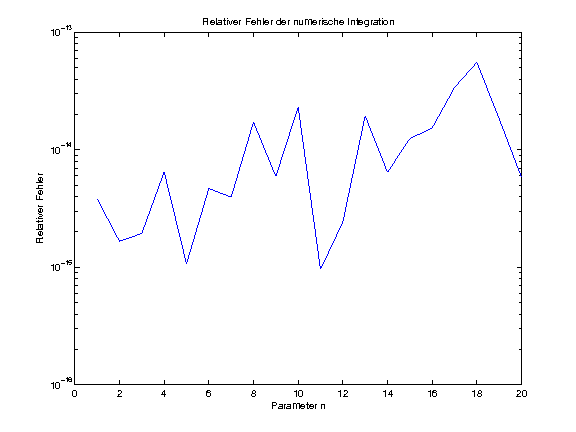
\includegraphics[scale=0.6]{fehler.png}
\end{figure}
\end{description}

Es gibt in matlab ebenfalls Funktionen wie quadl, quadgk und quadv. Allerdings könnte ich auch nur aus dem matlab-Tutorial abschreiben, wann welche Funktion besser ist...

\newpage
%% ------------------------------------------------------
%%                     AUFGABE 2
%% ------------------------------------------------------

\section*{Ausgabe 2}
\begin{description}
\item[a)] Z.z. Newton-Cotes-Formeln symmetrisch, d.h. für die Gewichte gilt: $\lambda_k = \lambda_{n-k}$ für alle $n$. \\
\begin{eqnarray*}
 \lambda_k &=& \frac{1}{n} \int_0^n{\prod_{j=0,j\neq k}^n{\frac{s-j}{k-j}} \, ds} \\
 &=&\frac{1}{n} \int_0^n{\frac{s-0}{k-0}\cdot \ldots \cdot \frac{s-(k-1)}{k-(k-1)} \cdot \frac{s-(k+1)}{k-(k+1)}\cdot \ldots \cdot \frac{s-n}{k-n} \, ds} \\
 & & \text{Substitution } t = n - s, \text{ also } dt = -ds\\
 &=&\frac{1}{n} \int_0^n{\frac{n-t}{k-0}\cdot \ldots \cdot \frac{n-t-(k-1)}{k-(k-1)} \cdot \frac{n-t-(k+1)}{k-(k+1)}\cdot \ldots \cdot \frac{n-t-n}{k-n} \, dt} \\
 &=&\frac{1}{n} \int_0^n{\frac{n-t}{k}\cdot \ldots \cdot \frac{n-t-k+1}{1} \cdot \frac{n-t-k-1}{-1}\cdot \ldots \cdot \frac{-t}{k-n} \, dt} \\
 &=&\frac{1}{n} \int_0^n{\frac{t-n}{-k}\cdot \ldots \cdot \frac{t-n+k-1}{-1} \cdot \frac{t-n+k+1}{1}\cdot \ldots \cdot \frac{-t}{k-n} \, dt} \\
 &=&\frac{1}{n} \int_0^n{\frac{t-n}{-k}\cdot \ldots \cdot \frac{n-t-k+1}{1} \cdot \frac{n-t-k-1}{-1}\cdot \ldots \cdot \frac{t}{n-k} \, dt} = \lambda_{n-k}\\
\end{eqnarray*}
\item[b)] Z.z. $\sum_{k=0}^{n}{\lambda_k} = 1, n\in \mathbb{N}$. \\
Die Interpolationspolynome sind so konstruiert, dass Funktionen vom Grad $\leq n$ mit ihrem Interpolationspolynom übereinstimmen.\\
Wir können die rechte Seite der Gleichung als konstate 1-Funktion betrachten. Da der Grad der 1-Funktion 0 ist, und $0 \leq n$, so ist das Interpolationspolynom ebenfalls identisch gleich 1, also $1 \equiv p_n(x_i) = f(x_i) = 1$. Da das bestimmte Integral der 1-Funktion von $a$ bis $b$ genau $(b-a)$ ist, liefert
$$ I_n(1) = (b-a) \sum_{k=0}^n{f(x_k)\lambda_k} = (b-a) \sum_{k=0}^n{\lambda_k} = (b-a)$$
$ \Rightarrow \sum_{k=0}^n{\lambda_k}= 1$.

\end{description}
%% ------------------------------------------------------
%%                     AUFGABE 3
%% ------------------------------------------------------

\section*{Ausgabe 3}
nö :)

\label{LastPage}

\end{document}
